\documentclass{beamer}

% You can also use a 16:9 aspect ratio:
%\documentclass[aspectratio=169]{beamer}
\usetheme{TACC16}

% It's possible to move the footer to the right:
%\usetheme[rightfooter]{TACC16}

%% page 
%\begin{frame}{}
%  \begin{itemize}
%    \item
%  \end{itemize}
%\end{frame}
%
%% page 
%\begin{frame}[fragile]
%    \frametitle{}
% {\tiny
%    \begin{semiverbatim}
%    \end{semiverbatim}
%}
%  \begin{itemize}
%    \item
%  \end{itemize}
%
%\end{frame}
 
\begin{document}
\title[Lmod]{15 years of Lmod: A Retrospective}
\author{Robert McLay} 
\date{August 1, 2023}

% page 1
\frame{\titlepage} 


% page 2
\begin{frame}{Outline}
  \center{\includegraphics[width=.9\textwidth]{Lmod-4color@2x.png}}
  \begin{itemize}
    \item The start of Lmod
    \item Why I used Lua to implement Lmod?
    \item Where Lmod success comes from?
    \item Features added over time
    \item Lmod lessons learned
    \item Conclusions
  \end{itemize}
\end{frame}

% page 3
\begin{frame}{The start of Lmod}
  \begin{itemize}
    \item In 2008, my friend and colleague Bill Barth asked:
    \item TACC has a software hierarchy with Tmod 3.2.10 (TCL/C)
    \item Impossible to change compilers or mpi modules
    \item Help?
  \end{itemize}
\end{frame}

% page 4
\begin{frame}{Key Insight}
  \begin{itemize}
    \item Remember the state of \$MODULEPATH
    \item When it changes, change loaded modules if necessary
    \item Support the idea of inactive modules
    \item Lmod was born
  \end{itemize}
\end{frame}

% page 5
\begin{frame}{Why implement in Lua?}
  \begin{itemize}
    \item TCL is not my favorite language
    \item TCL/C Tmod was/is very complicated (and ugly!!)
    \item Worked in Lua to develop testing tools (more on this latter)
    \item Did consulting work in Python before TACC: Avoid conflicts
    \item If useful, the idea would be integrated into Tmod (Nope!)
    \item Happy accident: Lua is fast enough
    \item Lua is easier to protect from user environments (Esp. Python)
  \end{itemize}
\end{frame}

% page 6
\begin{frame}{Some Reasons for Lmod Success}
  \begin{itemize}
    \item Initially no real competition (Tmod 4 started in 2017)
    \item Working at TACC helped
    \item Good enough documentation
    \item Easy transition from Tmod to Lmod (Lmod reads TCL
      modulefiles (Almost always works!?))
    \item Many Features not provided by other tools
    \item Unsolicited articles written by Jeff Layton about Lmod
    \item Many say: ``It just works so I don't worry about it.''
    \item Now used by EasyBuild, OpenHPC and Spack
    \item Packages for Mac Brew, Fedora, Debian
    \item It is reliable.
  \end{itemize}
\end{frame}

% page 7
\begin{frame}{Hidden Reason for Lmod Success}
  \begin{itemize}
    \item Testing Lmod has an extensive test suite (1400+ tests)
    \item Lmod uses the release early and often model.
    \item Almost 7000 check-in, 611 tags (versions)
    \item Can debug (via ml -D ... or ml -T) remotely
    \item My background is in 3-D Finite Element in C++
    \item I am a big fan of Design Patterns
    \item Lmod uses Singleton, Factories and Template pattern
      through-out for a code written in Lua.
  \end{itemize}
\end{frame}

% page 8
\begin{frame}{More on Testing}
  \begin{itemize}
    \item The TM testing suite filters output to converts to canonical
      names
    \item Makes output path independent so tests can be run anywhere
    \item Tests both stderr and stdout output for each test
    \item Can repeatedly run a single test file or just the ones that
      failed
    \item Lmod is reliable because of testing
    \item Github Actions run tests on 4 version of Lua on both
      Ubuntu and macOS for every check-in. (Thanks Kenneth Host and
      Ward Poelmans!)
    \item There are also unit tests and installed Lmod set of tests
  \end{itemize}
\end{frame}

% page 9
\begin{frame}{Building trust with the user community}
  \begin{itemize}
    \item Making it reliable (again via Testing)
    \item Timely answering the email and github issues 
    \item Book: Team Geek
    \item Learning to be polite when answering and re-answering
      questions
    \item ``You might consider ...''
    \item ``Please test Lmod version ... when you get a chance to see
      if it works for you''
    \item Not getting upset when non-native English speakers sound
      insulting
  \end{itemize}
\end{frame}

% page 10
\begin{frame}{Features addesd over time}
  \begin{itemize}
    \item Tab completion for bash and z-shell
    \item Support for N/V then C/N/V finally N/V/V (Lmod 7+)
    \item Sematic versioning (5.9 $<$ 5.10)
    \item Module properties
    \item Spider cache (speed up ``module avail'' and ``module load'')
    \item Personal Collections
    \item ml
    \item sandbox (prevents modulefiles from calling internal routines)
  \end{itemize}
\end{frame}

% page 11
\begin{frame}{Features part II}
  \begin{itemize}
    \item pushenv, sticky modules, i18n error messages
    \item Hooks, /etc/lmod/lmod\_config.lua
    \item Tracking of module usage via hooks
    \item Hidden modules
    \item depends\_on()
    \item source\_sh(): source a shell script inside a modulefile
    \item LMOD\_QUARANTINE\_VARS
    \item ...
  \end{itemize}
\end{frame}

% page 12
\begin{frame}{Lmod lesson learned}
  \begin{itemize}
    \item A private repo (bitbucket) as well as a public repo (github)
    \item make gittag TAG=...; make world\_update
    \item git worktrees
    \item Exploiting Lmod to help XALT
    \item Learned way more than I ever wanted to know about bash, zsh,
      tcsh shell startup procedures
    \item Want tcsh to die, die, die
    \item That default interactive non-login bash shell startup is
      borked (We patch bash to get to work)
    \item Can be difficult to decide what a user is reporting.  Bug or
      not?
    \item Getting users to use the bugReport script when submitting a
      bug.
  \end{itemize}
\end{frame}

% page 13
\begin{frame}{Lmod lesson learned (II)}
  \begin{itemize}
    \item That \texttt{module() \{ eval "\$(LMOD\_CMD bash "\$@")" \}}
        works better than
      \item \texttt{module() \{ eval \$(LMOD\_CMD bash "\$@") \}} who
        knew?
      \item Cannot test every possibility, users will \textbf{ALWAYS}
        find a case I missed
      \item The moduleTable has been incredible notion to store
        the module state in your env.
      \item That other tools will use the spider cache output.
      \item No two site are run exactly the same way.
      \item There are ten or more ways that Lmod can be tailored.
      \item Communicating changes thru README.new
  \end{itemize}
\end{frame}

% page 14
\begin{frame}[fragile]
    \frametitle{Lmod Doc usage by City}
    \center{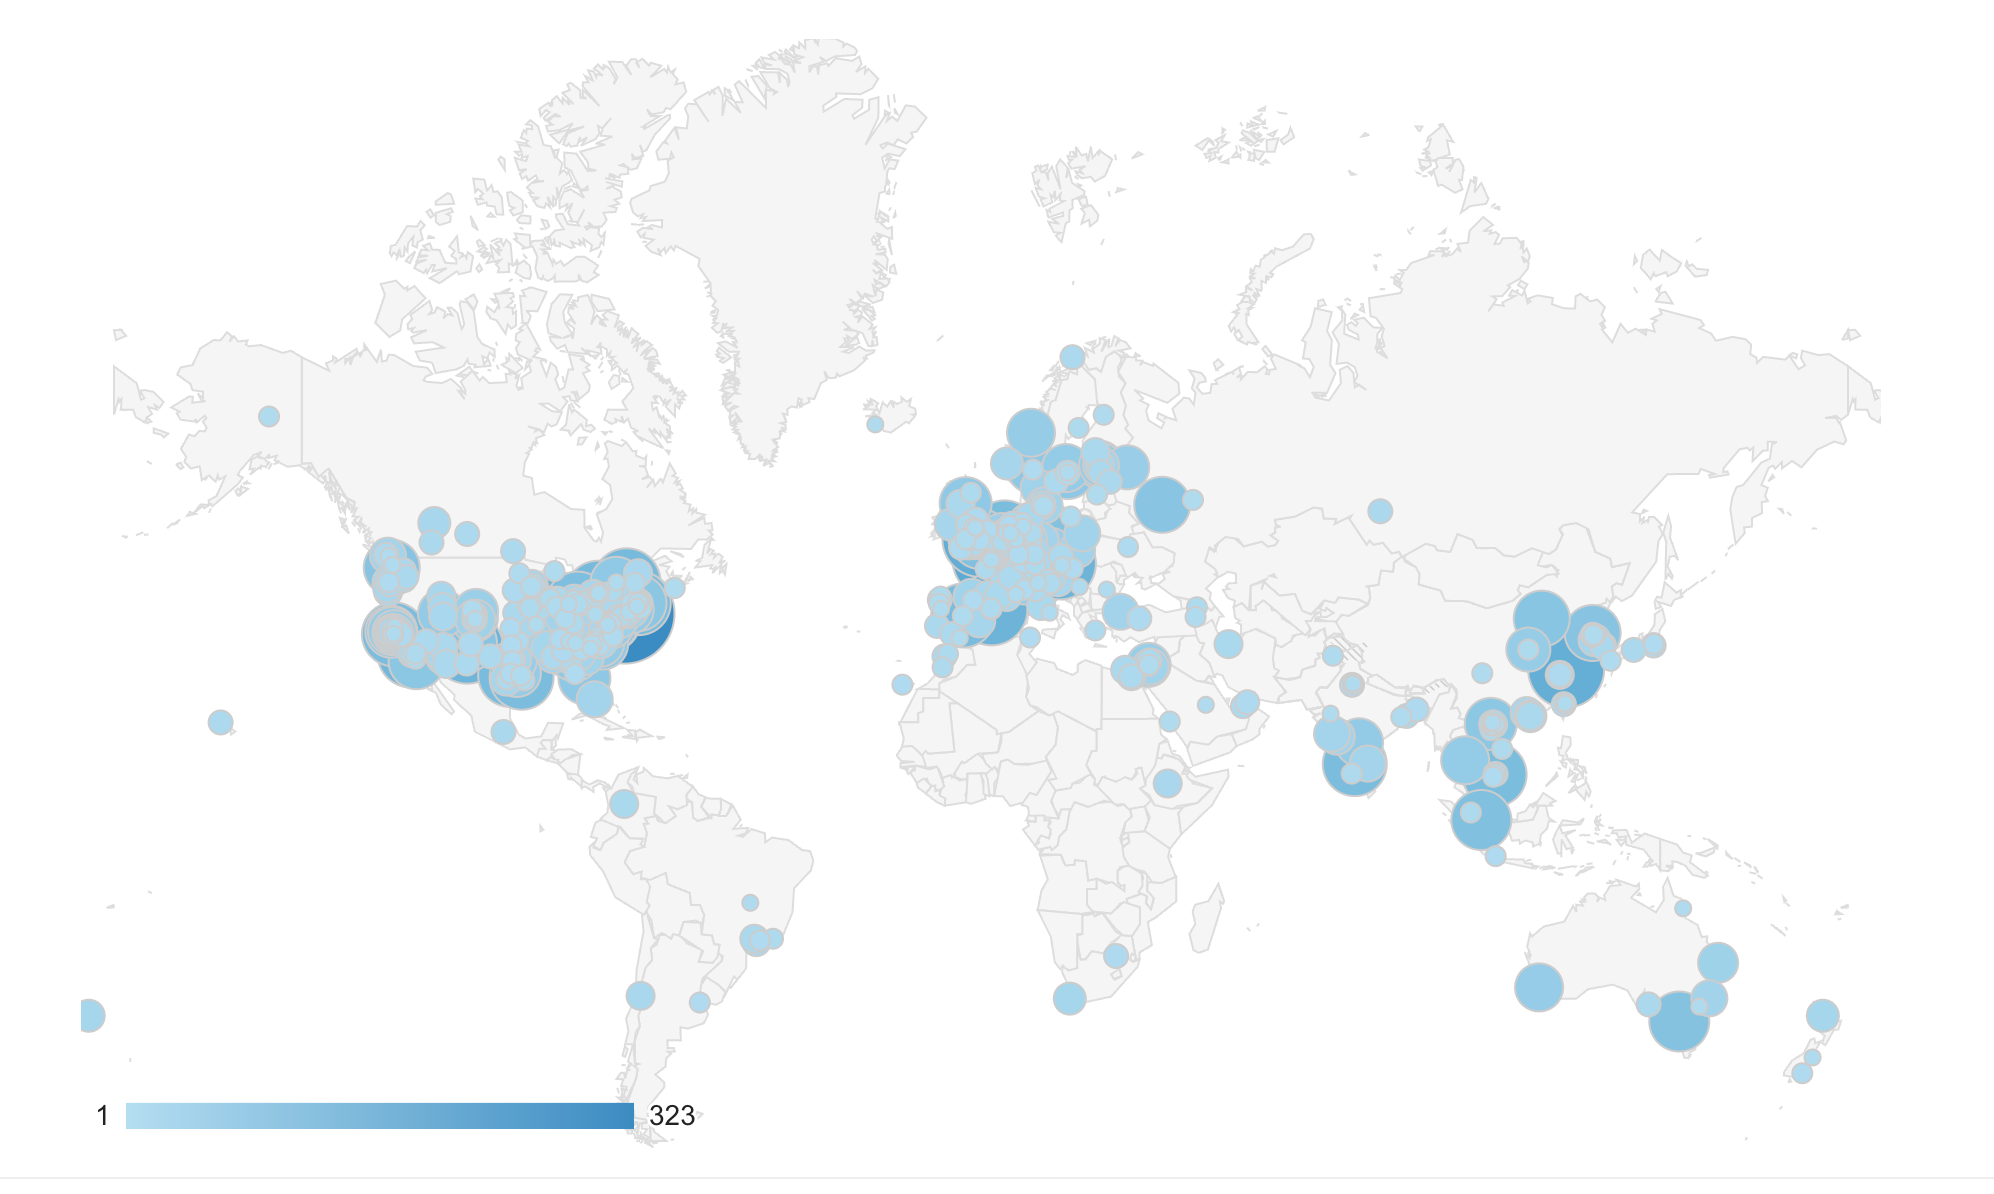
\includegraphics[width=.9\textwidth]{Lmod_doc_usage_by_city}}
\end{frame}

% page 15
\begin{frame}{Conclusions}
  \begin{itemize}
    \item Not every site works like TACC.
    \item That making Lmod available to the world has made it so much
      better.
    \item I have made many friends over the years through working on Lmod.
    \item Working on Lmod has been a fun part of the job.
    \item I have been giving these Lmod Monthly talks since Sept 2021
  \end{itemize}
\end{frame}


% page 16
\begin{frame}{Future Topics}
  \begin{itemize}
    \item Next Meeting will be Sept. 5th at 9:30 Central (14:30 UTC)
    \item Mathew Cawood will be running the meeting with a different
      zoom link
  \end{itemize}
\end{frame}

\end{document}
